\begin{figure}
    \centering
    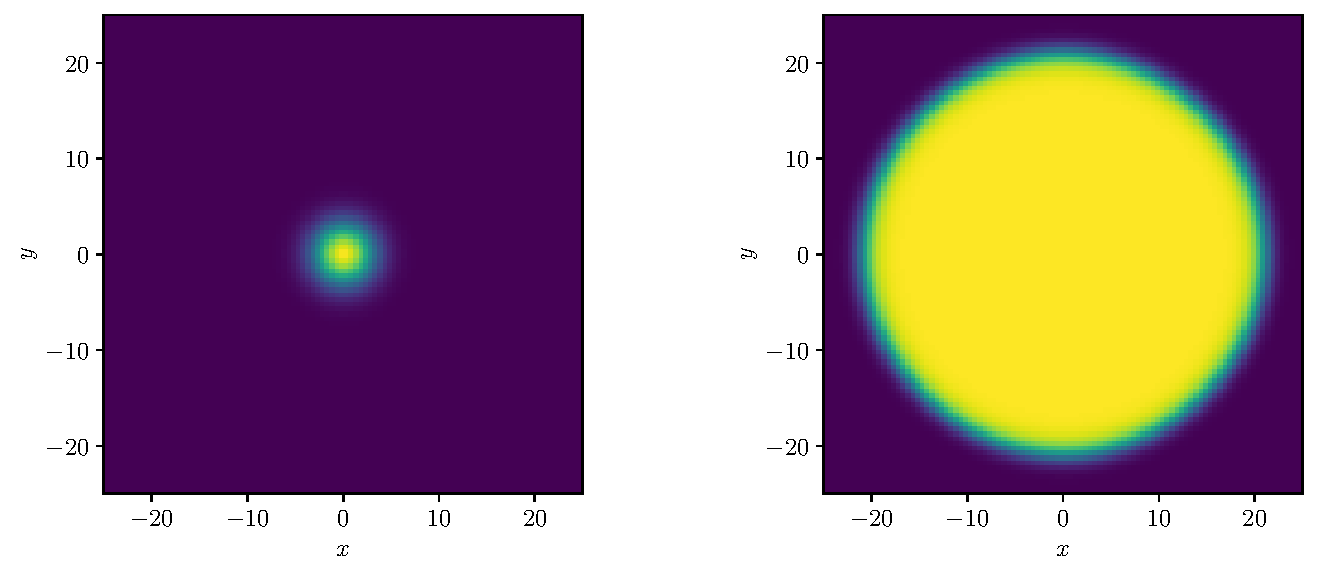
\includegraphics[width=\textwidth]{papers/reaktdiff/images/Fisher_KPP/fisher_kpp_2d_wave_comparison.pdf}
    \caption{Simulation der Fisher-KPP-Gleichung mit \(D = 0.1\) und \(r = 1\). Die Welle breitet sich mit einer Geschwindigkeit von \(v = 0.01\) aus. Das linke Bild zeigt die Simulation zum Zeitpunkt \(t = 0\) und das rechte Bild zum Zeitpunkt \(t = 25\).}
    \label{reaktdiff:figure:fisher_kpp_simulation}
\end{figure}
